\subsubsection{Example Unification}

Suppose we want to join two states of a FunArray \texttt{\string{0 i\string} $\top$ \string{n\string}} and \texttt{\string{0 i-1\string} [0,0] \string{1 i\string} $\top$ \string{n\string}?}, as in \cite[example 8]{cousot2011}. The neutral elements for the join operation are $\nElement_l=\nElement_r=\bot$ The following diagram displays the arrays as little bars. The segment values are inside the bars and the bounds can be found below. Potentially empty segments have dashed outlines.

\vspace{0.2cm}
\begin{center}
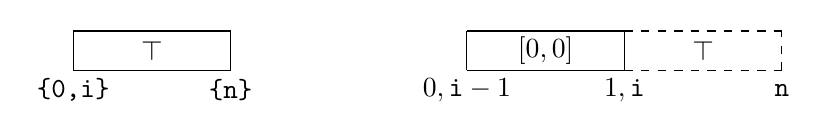
\begin{tikzpicture}
    \draw (0,0) -- (2,0);
    \draw (0,0.5) -- (2,0.5);

    \draw (0,0) -- (0,0.5);
    \draw (0,-0.25) node {\texttt{\string{0,i\string}}};

    \draw (1,0) node[anchor=south] {$\top$};

    \draw (2,0) -- (2,0.5);
    \draw (2,-0.25) node {\texttt{\string{n\string}}};


	\draw (5,0) -- (7,0);
    \draw (5,0.5) -- (7,0.5);

    \draw (5,0) -- (5,0.5);
    \draw (5,-0.25) node {$0, \mathtt{i}-1$};

    \draw (6,-0.05) node[anchor=south] {$[0,0]$};

	\draw (7,0)[dashed] -- (9,0);
    \draw (7,0.5)[dashed] -- (9,0.5);

    \draw (7,0) -- (7,0.5);
    \draw (7,-0.25) node {$1, \mathtt{i}$};

	\draw (8,0) node[anchor=south] {$\top$};

	\draw (9,0)[dashed] -- (9,0.5);
    \draw (9,-0.25) node {$\mathtt{n}$};    
\end{tikzpicture}
\end{center}


\noindent Let us restrict the expressions to those appearing in both FunArrays as in step~\ref{item:restrictexpressions}.


\vspace{0.2cm}
\begin{center}
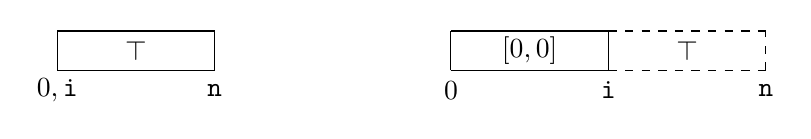
\begin{tikzpicture}
    \draw (0,0) -- (2,0);
    \draw (0,0.5) -- (2,0.5);

    \draw (0,0) -- (0,0.5);
    \draw (0,-0.25) node {$0, \mathtt{i}$};

    \draw (1,0) node[anchor=south] {$\top$};

    \draw (2,0) -- (2,0.5);
    \draw (2,-0.25) node {$\mathtt{n}$};


	\draw (5,0) -- (7,0);
    \draw (5,0.5) -- (7,0.5);

    \draw (5,0) -- (5,0.5);
    \draw (5,-0.25) node {$0$};

    \draw (6,-0.05) node[anchor=south] {$[0,0]$};

	\draw (7,0)[dashed] -- (9,0);
    \draw (7,0.5)[dashed] -- (9,0.5);

    \draw (7,0) -- (7,0.5);
    \draw (7,-0.25) node {$\mathtt{i}$};

	\draw (8,0) node[anchor=south] {$\top$};

	\draw (9,0)[dashed] -- (9,0.5);
    \draw (9,-0.25) node {$\mathtt{n}$};    
\end{tikzpicture}
\end{center}


\noindent This leaves no empty bounds, meaning we can proceed with step \ref{item:traverse}. We examine the first bound of both FunArrays. Since \texttt{\string{0,i\string}}